\documentclass[11pt,a4paper]{article}

\usepackage[a4paper,top=2.5cm,bottom=2.5cm,left=2cm,right=2cm]{geometry}
\usepackage{fontspec}
\usepackage{xeCJK}
\setmainfont{Times New Roman}
\IfFontExistsTF{Microsoft YaHei}{\setCJKmainfont{Microsoft YaHei}\setCJKmonofont{Microsoft YaHei}}{\setCJKmainfont{SimSun}\setCJKmonofont{SimSun}}
\usepackage{amsmath,amssymb}
\usepackage{xcolor}
\usepackage{enumitem}
\usepackage{titlesec}
\usepackage{graphicx}
\usepackage{float}
\usepackage{booktabs}
\usepackage{tabularx}
\usepackage{array}
\usepackage{hyperref}
\hypersetup{colorlinks=true,linkcolor=blue,citecolor=blue,urlcolor=blue}

\definecolor{commentgray}{RGB}{90,90,90}
\definecolor{locationblue}{RGB}{22,73,140}
\newenvironment{reviewercomment}{\begin{quote}\small\itshape\color{commentgray}}{\end{quote}}
\newcommand{\authorresponse}{\noindent\textbf{作者回复：}\quad}
\newcommand{\revisionlocation}[1]{\par\noindent\textcolor{locationblue}{\textbf{修改位置：}}#1}
\newcommand{\draftplaceholder}[1]{\textcolor{red}{\textbf{[待完成：#1]}}}
\renewcommand{\tablename}{表}
\renewcommand{\figurename}{图}
\titleformat{\section}{\large\bfseries}{}{0pt}{}
\titleformat{\subsection}{\normalsize\bfseries}{}{0pt}{}
\setlength{\parindent}{0pt}
\setlength{\parskip}{0.45em}

\begin{document}

\begin{center}
{\LARGE\textbf{审稿意见回复信 (Response Letter)}}\\[1em]
\textbf{稿件编号：}NETJOURNAL-D-26-00829\\
\textbf{论文题目：}\parbox[t]{0.82\textwidth}{\centering A deep-learning method based on the variable-domain integral weak-solution formulation for neutron diffusion equations with piecewise material coefficients}\\[0.5em]
\textbf{投稿期刊：}Nuclear Engineering and Technology\\[0.5em]
% AUTOFILL:ZH_STATUS:BEGIN
\textbf{当前状态：}\textcolor{red}{\texttt{draft\_with\_placeholders}}
% AUTOFILL:ZH_STATUS:END
\end{center}

\vspace{1em}
尊敬的编辑与审稿专家：

% AUTOFILL:ZH_INTRO:BEGIN
我们诚挚感谢编辑和两位审稿专家对稿件的认真评阅。我们根据意见重新定位了论文贡献，补充了 VIWS 与原函数网络的数学和实现细节，重写了摘要，完善了网络、损失函数、优化流程、采样方式和特征值联合求解说明，并增加了三维轴向平均结果、二维/三维 PINN--VIWS 纯推理测试及 2D-IAEA 分辨率推理内存测试。对于尚未完成的二维和三维 PINN--VIWS 三次独立训练比较，我们在正文和本回复中保留了误差与训练时间占位符，不会在获得真实服务器日志前填写或提交相关数值。
% AUTOFILL:ZH_INTRO:END

以下逐条保留审稿意见原文，并说明相应修改及其在修订稿中的位置。

\section*{针对审稿人 \#1 的回复}

\subsection*{R1.P -- 审稿人总体评价}
\begin{reviewercomment}
本文提出了一种用于求解非均匀介质中中子扩散方程的深度学习框架。本文所处理的主要挑战是材料界面处存在不连续的扩散系数和宏观截面。这些不连续性会引起通量梯度跳跃和界面奇异性，可能对基于神经网络的求解器的精度与收敛性产生不利影响。为解决这一问题，作者采用变域积分弱解（Variable-Domain Integral Weak Solution, VIWS）方法建立中子扩散方程，并使用单网络表示全局解。该方法旨在无需显式处理内部材料界面的情况下求解非均匀中子扩散问题。该主题与反应堆物理中深度学习方法的应用相关，并具有潜在价值。然而，稿件缺少足够的方法与实现细节，读者尚难以充分理解、复现和评价所提出的方法。以下意见需要处理。
\end{reviewercomment}
% AUTOFILL:ZH_R1P:BEGIN
\authorresponse 感谢审稿专家的这些意见。针对可理解性、可复现性和可评价性不足的问题，我们已明确说明 VIWS 数学形式及其如何嵌入标准全连接网络，补充完整损失函数和训练伪代码，说明各网络的输入、输出与物理角色，并扩展数值证据和局限性讨论。尚未完成的同条件训练成本数据仍以醒目占位符标出，在取得经核验日志前不会填写。
% AUTOFILL:ZH_R1P:END
相应修改见第 \draftplaceholder{页码} 页（第 \draftplaceholder{行号} 行）。
\revisionlocation{标题；摘要；第 3.3--3.4 节；第 4 节；结论。}

\subsection*{R1.1 -- 意见 1}
\begin{reviewercomment}
摘要没有清楚说明比较基线。建议明确指出所提出的方法是与传统 PINN、有限元方法（FEM）、有限差分方法（FDM），还是其他成熟的中子扩散求解器进行比较。此外，摘要没有说明计算成本、训练时间、内存需求，或向大规模反应堆计算扩展的能力。
\end{reviewercomment}
% AUTOFILL:ZH_R11:BEGIN
\authorresponse 感谢审稿专家的这些意见。我们已经完全重写摘要，并明确区分两类基线：有限元解仅作为高精度参考解，标准 PINN 作为神经网络定量比较基线。摘要现已给出二维六边形、三维八区域和 2D-IAEA 算例的代表性误差。我们完成了共同通量网络在 10,000 个二维坐标和 216,000 个三维坐标上的纯推理测试，并完成了 2D-IAEA 在 $100^2$ 至 $800^2$ 查询网格上的推理时间和峰值 GPU 显存测试。二维、三维三次独立训练的误差统计与训练时间尚未完成，因此目前保留明确占位符，也未声称 VIWS 快于传统求解器。
% AUTOFILL:ZH_R11:END
相应修改见第 \draftplaceholder{页码} 页（第 \draftplaceholder{行号} 行）。
\revisionlocation{摘要；第 4 节开头；新增“PINN--VIWS 计算成本比较表”和“2D-IAEA 分辨率推理内存表”。}

\subsection*{R1.2 -- 意见 2}
\begin{reviewercomment}
稿件应更详细地讨论所提出方法中原函数形式所涉及的存在性与唯一性条件。
\end{reviewercomment}
\authorresponse 感谢审稿专家的这些意见。修订稿首先用具有固定下限的重复积分给出连续核函数原函数的显式构造，从而说明其存在性。我们进一步说明，仅给出全混合偏导关系时原函数并不唯一。本文按照已有 VIWS 理论文献，在仿射修正族内选取代表元：二维使用 3 个不共线确定点，三维使用 4 个不共面确定点，以唯一确定仿射修正系数。我们特别强调，该唯一性结论仅适用于所选仿射修正族，并非一般函数空间中的全局唯一性。不连续材料反应核不强行构造全局原函数，而采用按材料区域分段积分。相应修改见第 \draftplaceholder{页码} 页（第 \draftplaceholder{行号} 行）。
\revisionlocation{第 3.3 节“Antiderivative transformation”，新增仿射原函数族公式及其后讨论。}

\subsection*{R1.A -- 原决定信中未编号的网络结构意见}
\begin{reviewercomment}
稿件对神经网络结构的描述不够充分。如果分别使用原函数网络和中子通量网络，应明确说明它们的结构。至少应提供以下信息：
\begin{enumerate}[label=\alph*.,leftmargin=2em]
\item 网络结构；
\item 隐藏层数量；
\item 每层神经元数量；
\item 激活函数；
\item 输入/输出变量；
\item 训练策略。
\end{enumerate}
\end{reviewercomment}
\authorresponse 感谢审稿专家的这些意见。我们已经补充完整的网络结构和训练说明。每个能群使用一个覆盖全计算域的通量网络；“global network”并不表示整个多群求解器只有一个网络。通量网络使用 8 个隐藏层，每层 32 个神经元；各原函数辅助网络使用 6 个隐藏层，每层 32 个神经元；两者均采用 Tanh，隐藏层数不含输入层和输出层。二维和三维输入分别为空间坐标 $(x,y)$ 和 $(x,y,z)$，每个网络输出一个标量场。训练采用 Adam 后接 L-BFGS 的两阶段策略。

为便于审稿专家快速核对，我们将修订稿中补充的关键实现信息汇总如下。

\begin{table}[H]
\centering
\small
\caption{修订稿新增的关键网络角色与训练设置。}
\label{tab:response_network_settings_zh}
\renewcommand{\arraystretch}{1.15}
\begin{tabularx}{0.98\textwidth}{@{}p{2.7cm}p{2.6cm}p{2.4cm}X@{}}
\toprule
组成部分 & 输入/输出 & 网络结构 & 物理角色与训练方式 \\
\midrule
通量网络 & 空间坐标/标量中子通量 & 8 个隐藏层 $\times$ 32，Tanh & 每个能群使用一个全域网络；采用 Adam 后接 L-BFGS 优化。 \\
原函数网络 & 空间坐标/标量辅助场 $F_k$ & 6 个隐藏层 $\times$ 32，Tanh & 在固定源算例中表征连续 VIWS 核，并与通量网络联合优化。 \\
特征值实现 & 坐标/两个能群标量通量；全局 $k_{\mathrm{eff}}$ & 两个 8 $\times$ 32 通量网络 & 两群网络与 $k_{\mathrm{eff}}$ 联合优化；结构化网格 IAEA 算例直接采用累积数值积分。 \\
\bottomrule
\end{tabularx}
\end{table}
相应修改见第 \draftplaceholder{页码} 页（第 \draftplaceholder{行号} 行）。
\revisionlocation{第 3.4 节；新增网络与优化设置表。}

\subsection*{R1.3 -- 意见 3}
\begin{reviewercomment}
优化过程的描述不够充分。稿件应清楚说明可训练参数、优化算法、学习率策略，以及训练过程中采用的其他优化设置。
\end{reviewercomment}
\authorresponse 感谢审稿专家的这些意见。我们已在正文中说明可训练变量包括通量网络参数、原函数网络参数，以及特征值问题中的全局标量 $k_{\mathrm{eff}}$。Adam 固定运行 2,000 次，初始学习率为 $10^{-3}$；随后使用 L-BFGS 精修。L-BFGS 的最大迭代数、历史长度、梯度容差、变化容差和 strong-Wolfe 线搜索均集中列入训练设置表。损失权重和 Fourier 特征矩阵固定不训练；若使用测试函数网络，则先预训练并在主求解阶段冻结。相应修改见第 \draftplaceholder{页码} 页（第 \draftplaceholder{行号} 行）。
\revisionlocation{第 3.4 节；新增 VIWS 训练伪代码和网络与优化设置表。}

\subsection*{R1.4 -- 意见 4}
\begin{reviewercomment}
稿件称，当损失达到预设精度要求或满足停止准则时终止训练。然而，文中既没有明确定义该精度要求，也没有明确定义停止准则。稿件引用参考文献 38 和 39 说明这些细节，但其中一篇文献不便于国际读者获取，因此相关信息应直接写入稿件。
\end{reviewercomment}
% AUTOFILL:ZH_R14:BEGIN
\authorresponse 感谢审稿专家的这些意见。我们已删除未定义的“preset accuracy requirement”。Adam 在 2,000 次迭代后停止；L-BFGS 在达到最大迭代数、梯度容差或参数/目标函数变化容差之一时停止。修订稿直接给出这些规则，不再要求读者查阅外部文献。各算例的实际停止轮数和最终损失将在统一重跑日志完成后填写。
% AUTOFILL:ZH_R14:END
相应修改见第 \draftplaceholder{页码} 页（第 \draftplaceholder{行号} 行）。
\revisionlocation{第 3.4 节；网络与优化设置表。\draftplaceholder{补入统一重跑后的实际停止轮数和最终损失。}}

\subsection*{R1.5 -- 意见 5}
\begin{reviewercomment}
术语 L-BFGS 在第 4 节出现之前没有介绍。作者应给出其全称，并简要说明它在优化过程中的作用。
\end{reviewercomment}
\authorresponse 感谢审稿专家的这些意见。我们已在首次出现处写出 limited-memory Broyden--Fletcher--Goldfarb--Shanno (L-BFGS) algorithm，并说明其作用是在 Adam 获得稳定初值后利用有限内存拟牛顿更新进一步降低耦合损失。我们没有对其作全局收敛性宣称。相应修改见第 \draftplaceholder{页码} 页（第 \draftplaceholder{行号} 行）。
\revisionlocation{第 3.4 节训练说明。}

\subsection*{R1.6 -- 意见 6}
\begin{reviewercomment}
稿件称“默认网络为 8 层 FCNN”。应澄清“默认”的含义：该结构是否用于全部数值实验，还是仅在没有另行说明时使用？
\end{reviewercomment}
\authorresponse 感谢审稿专家的这些意见。我们已删除“default network”这一含混表述，并统一说明所有报告算例使用的通量网络和原函数网络结构，同时明确层数不包括输入层与输出层。相应修改见第 \draftplaceholder{页码} 页（第 \draftplaceholder{行号} 行）。
\revisionlocation{第 3.4 节；网络与优化设置表；第 4 节开头。}

\subsection*{R1.7 -- 意见 7}
\begin{reviewercomment}
稿件应明确说明每个神经网络所用输入和输出变量的数量及其物理含义。
\end{reviewercomment}
\authorresponse 感谢审稿专家的这些意见。修订稿现已逐类说明网络变量。通量网络仅输入空间坐标并输出相应能群的标量通量；每个原函数网络输入相同坐标并输出一个标量辅助场。材料系数和外源由坐标查询后进入残差，但不是网络输入。Fourier 特征只是坐标的固定映射。$k_{\mathrm{eff}}$ 是独立全局可训练标量，不是空间网络的输入或输出。相应修改见第 \draftplaceholder{页码} 页（第 \draftplaceholder{行号} 行）。
\revisionlocation{第 3.4 节，通量网络与原函数网络定义公式后的说明。}

\subsection*{R1.8 -- 意见 8}
\begin{reviewercomment}
稿件没有充分解释如何将 VIWS 形式纳入深度学习框架。需要清楚指出 VIWS 形式在神经网络训练过程中的具体作用位置，以及它如何构成损失函数或控制约束。
\end{reviewercomment}
\authorresponse 感谢审稿专家的这些意见。我们已补充完整损失定义和训练伪代码。VIWS 直接定义控制方程残差 $\mathcal L_{\mathrm r}$，并与原函数定义损失 $\mathcal L_{\mathrm{def}}$、确定点损失 $\mathcal L_F$、边界损失 $\mathcal L_{\mathrm b}$ 以及特征值归一化损失 $\mathcal L_{\mathrm{norm}}$ 共同反向传播。修订稿还逐步列出从采样、通量及梯度计算、核函数构造、分段积分到联合更新的过程。相应修改见第 \draftplaceholder{页码} 页（第 \draftplaceholder{行号} 行）。
\revisionlocation{第 3.4 节，新增的五类损失公式和 VIWS 训练伪代码。}

\subsection*{R1.9 -- 意见 9}
\begin{reviewercomment}
目前尚不完全清楚中子扩散方程是通过 VIWS 形式导出的积分残差来施加约束，还是通过其他实现方式施加约束。应澄清这一点。
\end{reviewercomment}
\authorresponse 感谢审稿专家的这些意见。本文控制方程通过 VIWS 变域积分残差约束，而不是使用原中子扩散方程的强形式残差。连续扩散核和边界核由原函数网络及自动微分表示；含分片吸收、散射、裂变和外源参数的项按材料区域分段积分。本文未增加显式内部界面惩罚项。相应修改见第 \draftplaceholder{页码} 页（第 \draftplaceholder{行号} 行）。
\revisionlocation{第 3.3--3.4 节；VIWS 控制式及总损失后的实现说明。}

\subsection*{R1.10 -- 意见 10}
\begin{reviewercomment}
“在深度学习求解中使用原函数形式”之类的表述使读者难以理解。稿件应更明确地解释如何把原函数形式纳入训练过程，以及该形式如何影响计算效率。
\end{reviewercomment}
\authorresponse 感谢审稿专家的这些意见。我们已明确说明：原函数网络的混合偏导通过 $\mathcal L_{\mathrm{def}}$ 重构连续核，而原函数值本身进入 VIWS 方程残差 $\mathcal L_{\mathrm r}$。这种表示减少连续变上限积分的重复累计求积，但会增加辅助网络和自动微分开销。因此修订稿不再声称原函数变换必然提高效率，也没有把整体 VIWS--PINN 计时归因于单一组件。相应修改见第 \draftplaceholder{页码} 页（第 \draftplaceholder{行号} 行）。
\revisionlocation{第 3.3--3.4 节；结论的局限性段落。}

\subsection*{R1.11 -- 意见 11}
\begin{reviewercomment}
我认为本文并未提出新的神经网络架构，而是提出了一种嵌入深度学习框架的新数学形式（VIWS），以更好地处理非均匀中子扩散问题中的材料界面。如果确实如此，请在稿件中明确说明。
\end{reviewercomment}
\authorresponse 感谢审稿专家的这些意见。我们完全同意。标题、摘要、引言、方法和结论现已统一说明：本文贡献是嵌入标准全连接网络的 VIWS 数学控制形式及其实现方法，而不是一种新的神经网络架构。相应修改见第 \draftplaceholder{页码} 页（第 \draftplaceholder{行号} 行）。
\revisionlocation{标题；摘要；引言末段；第 3.4 节首段；结论首段。}

\subsection*{R1.12 -- 意见 12}
\begin{reviewercomment}
与传统中子扩散方程（NDE）求解器相比，该方法的执行时间和内存占用如何？
\end{reviewercomment}
% AUTOFILL:ZH_R112:BEGIN
\authorresponse 感谢审稿专家的这些意见。我们同意原稿没有提供足够证据支持速度相关表述。修订稿仅在同一硬件和共同最终通量网络下报告标准 PINN 与 VIWS 的纯推理成本，并把 FEM 作为高精度参考和定性讨论对象。二维 10,000 个查询点的中位推理时间分别为 0.00217~s 和 0.00208~s，峰值显存均为 14.221~MiB；三维 216,000 个查询点分别为 0.03914~s 和 0.03953~s，峰值显存均为 119.598~MiB。这些数据只表示部署阶段通量查询，不代表训练显存。由于尚未建立与成熟传统 NDE 求解器在同平台、同误差容限下的公平基准，我们明确删除了“VIWS 快于传统求解器”的结论。\draftplaceholder{二维和三维 PINN--VIWS 三次独立训练的相对误差统计与训练时间仍需由服务器运行填入。}
% AUTOFILL:ZH_R112:END

为使成本修改能够直接核对，而不必在论文中来回查找，我们把最关键的同条件比较量列于下表。红色项目将在 12 次服务器运行完成并核验后自动回填，目前明确保留为未完成项。

\begin{table}[H]
\centering
\scriptsize
\caption{修订稿中的同条件 PINN--VIWS 精度与成本比较。数值为三次运行的中位数[范围]。}
\label{tab:response_matched_cost_zh}
\renewcommand{\arraystretch}{1.15}
\begin{tabularx}{\textwidth}{@{}llXXXX@{}}
\toprule
算例 & 方法 & 相对 $L_2$ 误差 & 训练时间 & 推理时间 (s) & 峰值 GPU 显存 (MiB) \\
\midrule
% AUTOFILL:ZH_MATCHED_TABLE:BEGIN
二维六边形 & PINN & \textcolor{red}{TBD} & \textcolor{red}{TBD} & 0.00217 [0.00213, 0.00223] & 14.221 [14.221,14.221] \\
二维六边形 & VIWS & \textcolor{red}{TBD} & \textcolor{red}{TBD} & 0.00208 [0.00207, 0.00208] & 14.221 [14.221,14.221] \\
三维八区域 & PINN & \textcolor{red}{TBD} & \textcolor{red}{TBD} & 0.03914 [0.03905, 0.03926] & 119.598 [119.598,119.598] \\
三维八区域 & VIWS & \textcolor{red}{TBD} & \textcolor{red}{TBD} & 0.03953 [0.03833, 0.03982] & 119.598 [119.598,119.598] \\
% AUTOFILL:ZH_MATCHED_TABLE:END
\bottomrule
\end{tabularx}
\end{table}
相应修改见第 \draftplaceholder{页码} 页（第 \draftplaceholder{行号} 行）。
\revisionlocation{摘要末句；第 4 节开头；新增 PINN--VIWS 计算成本比较表；结论。}

\section*{针对审稿人 \#2 的回复}

\subsection*{R2.G1 -- 总体意见 1}
\begin{reviewercomment}
稿件标题略有误导。“非均匀中子扩散计算”究竟指什么？如果该方法需要进行跨材料均匀化（例如，每个棒元被均匀化，不再分别表示包壳、气隙、燃料和慢化剂区域），那么“非均匀”一词并不适用于本文，应改为更恰当的术语。
\end{reviewercomment}
\authorresponse 感谢审稿专家的这些意见。我们已将标题改为“A deep-learning method based on the variable-domain integral weak-solution formulation for neutron diffusion equations with piecewise material coefficients”。二维六边形算例显式区分燃料、包壳和慢化剂区域；三维棒束算例区分棒区与外部材料区；2D-IAEA 则采用组件均匀化两群常数。全文尽量用“piecewise-defined material coefficients”替代过宽的“heterogeneous”表述。相应修改见第 \draftplaceholder{页码} 页（第 \draftplaceholder{行号} 行）。
\revisionlocation{标题；摘要；引言；第 4.5 节建模尺度说明。}

\subsection*{R2.G2 -- 总体意见 2}
\begin{reviewercomment}
摘要的质量明显低于稿件正文。正文较为简洁，术语使用正确，整体上可以理解，但摘要未能很好地反映论文内容。摘要中的某些句子甚至难以理解，因此作者需要完全重写摘要并认真校对，使其质量与正文相匹配。
\end{reviewercomment}
\authorresponse 感谢审稿专家的这些意见。我们接受这一意见并完全重写了摘要。新摘要依次说明多区域模型中的分片参数、标准 PINN 的困难、VIWS 控制形式、连续核与不连续项的不同处理、FEM 与 PINN 的角色、二维/三维/IAEA 定量结果，以及适用范围和速度结论边界。相应修改见第 \draftplaceholder{页码} 页（第 \draftplaceholder{行号} 行）。
\revisionlocation{摘要全文。}

\subsection*{R2.G3 -- 总体意见 3}
\begin{reviewercomment}
用 PINN 替代传统中子扩散求解器的一个重要方面，是其潜在的计算速度优势。所提出的方法与传统求解器进行严格同条件比较（使用完全相同数量的 CPU 核/GPU 卡和相同模型）时表现如何？如果更快，需要付出怎样的精度代价？内存消耗又如何？
\end{reviewercomment}
% AUTOFILL:ZH_R2G3:BEGIN
\authorresponse 感谢审稿专家的这些意见。我们同意应避免跨硬件、跨实现和跨误差容限的不公平比较。本文把定量成本比较限定为同条件的标准 PINN 与 VIWS，并明确 FEM 仅作为精度参考。二维和三维纯推理测试现已给出共同最终通量网络的时间与峰值显存；2D-IAEA 分辨率测试给出实际推理时间、峰值显存、输出数组内存和模型内存。本文不声称 VIWS 快于传统求解器；成熟 NDE 求解器的同平台比较列为后续工作。\draftplaceholder{补入二维、三维 PINN--VIWS 三次独立训练的相对误差统计与训练时间。}
% AUTOFILL:ZH_R2G3:END
相应修改见第 \draftplaceholder{页码} 页（第 \draftplaceholder{行号} 行）。
\revisionlocation{摘要；第 4 节开头；新增 PINN--VIWS 成本表和 2D-IAEA 内存表；结论。}

\subsection*{R2.G4 -- 总体意见 4}
\begin{reviewercomment}
尽管所提出的方法似乎很有价值，但稿件没有清楚说明其潜在缺点，因此读起来更像宣传材料；科学论文应同时呈现研究中观察到的优点与不足。
\end{reviewercomment}
\authorresponse 感谢审稿专家的这些意见。我们已重写结论并增加完整局限性段落，讨论每个新问题需要非凸重新训练、对采样和优化设置的敏感性、辅助网络和自动微分开销、不连续反应项仍需分段积分、复杂几何中的变量域与测试函数设计，以及当前验证尺度、边界类型、传统求解器基准和误差理论方面的限制。同时删除了多处宣传性和未经基准支持的效率表述。相应修改见第 \draftplaceholder{页码} 页（第 \draftplaceholder{行号} 行）。
\revisionlocation{结论第 3 段；摘要末句；第 4 节开头。}

\subsection*{R2.G5 -- 总体意见 5}
\begin{reviewercomment}
所提出的方法应以更具可复现性的方式介绍，而投稿稿件没有做到这一点。读者需要查阅文中提到的全部文献乃至更多资料，才能拼凑出实现类似求解器的具体流程。如果稿件能给出一个更直接的算法，说明作者如何构建模型、训练模型并在实际中使用，将会有很大帮助。还请作者注意，投稿期刊名为《Nuclear Engineering and Technology》。虽然稿件中的“Nuclear”很明确，但没有体现“Engineering”和/或“Technology”，使文章更像一份科学报告，而不是原创研究论文。请作者弥补这一差距。
\end{reviewercomment}
\authorresponse 感谢审稿专家的这些意见。我们已把方法改写为自包含实现：正文给出网络输入输出、五类损失、连续/不连续项的数据流、训练伪代码、统一网络结构、优化参数和停止规则。工程相关性通过 177 个组件位置的 2D-IAEA 组件均匀化基准、两群通量、22 pcm 特征值偏差和分辨率资源测试具体体现。修订稿不依赖未提供的代码仓库来解释算法，也不作代码公开承诺。相应修改见第 \draftplaceholder{页码} 页（第 \draftplaceholder{行号} 行）。
\revisionlocation{第 3.3--3.4 节；VIWS 训练伪代码；网络与优化设置表；第 4.5 节。}

\subsection*{R2.S1 -- 具体意见 1：摘要}
\begin{reviewercomment}
“中子扩散计算在反应堆物理中至关重要，但非均匀反应堆堆芯包含不连续的扩散系数和宏观截面。”

\begin{enumerate}[label=\alph*.,leftmargin=2em]
\item 看起来作者在一个发展已久的领域中引入了新的且不必要的术语。作者所谓“不连续”的扩散系数和“不连续”的宏观截面究竟是什么意思？在审稿人看来，这样的措辞组合没有意义。
\item 审稿人也不认同“反应堆堆芯包含这些系数或其他系数”的说法。作者需要校对整个摘要，以更加清楚、准确地表达观点。
\end{enumerate}
\end{reviewercomment}
\authorresponse 感谢审稿专家的这些意见。我们同意原句的主语和术语不准确，已经删除并改写为：“In multiregion neutron-diffusion models, each material region is represented by its own effective diffusion coefficient and macroscopic cross sections, and these piecewise-defined parameters may change abruptly across material interfaces.”该表述明确说明系数属于数学模型中的材料区域参数，而不是反应堆实体“包含系数”。相应修改见第 \draftplaceholder{页码} 页（第 \draftplaceholder{行号} 行）。
\revisionlocation{摘要首句；引言首段。}

\subsection*{R2.S2 -- 具体意见 2：图 4}
\begin{reviewercomment}
什么是原函数？为什么图 4 中的原函数场不对称？
\end{reviewercomment}
\authorresponse 感谢审稿专家的这些意见。我们已明确说明 $F$ 是用于重构积分核的非物理辅助标量，不是中子通量、功率或反应率。其代表元受积分方向、测试函数和确定点影响，因此即使物理通量具有对称性，$F$ 本身也不必具有相同对称性。需要满足的是其相应混合偏导重构目标核。图注现已列明 $F_0$、$F_1$、$F_2$ 的含义和确定点条件。相应修改见第 \draftplaceholder{页码} 页（第 \draftplaceholder{行号} 行）。
\revisionlocation{第 3.3--3.4 节；二维六边形原函数图图注。}

\subsection*{R2.S3 -- 具体意见 3：第 4.1 节}
\begin{reviewercomment}
“域内采样点和边界采样点的总数为 10,000。”

这些采样点是什么？具体如何使用？其数量是如何确定的，为什么这一数量很重要？
\end{reviewercomment}
\authorresponse 感谢审稿专家的这些意见。我们重新核对了实现，并更正了原先把 10,000 写成“域内点”的不准确表述。统一重跑协议使用 $100\times100$ 笛卡尔背景网格，即掩膜前共 10,000 个坐标；域损失只使用落在六边形内的有效点，每次运行会记录实际有效点数。另有 2,048 个沿六条边按弧长均匀分配且不重复顶点的边界点，以及每个原函数的 3 个二维确定点。标准 PINN 与 VIWS 在同一种子下使用完全相同的背景网格、域掩膜和边界点，且不进行界面加密。本文没有完成系统采样密度敏感性实验，因此已把该问题明确列为限制，而未声称当前点数具有普遍最优性。相应修改见第 \draftplaceholder{页码} 页（第 \draftplaceholder{行号} 行）。
\revisionlocation{第 4.1 节采样说明；结论局限性段落。}

\subsection*{R2.S4 -- 具体意见 4：第 4.3 节}
\begin{reviewercomment}
如果能给出轴向归一化图及其对比，将很有帮助。尤其应同时展示参考程序、PINN 和 VIWS 计算得到的通量图与源项图，而不只是通量图。
\end{reviewercomment}
\authorresponse 感谢审稿专家的这些意见。我们已增加 FEM、PINN 和 VIWS 的轴向平均通量及总源图。总源定义为 $q_{\mathrm{tot}}=S+\nu\Sigma_{\mathrm f}\phi$，所有方法对同一物理量均使用 FEM 轴向平均最大值统一归一化，并共享色标。轴向平均通量的 PINN 和 VIWS 相对 $L_2$ 误差分别为 $3.55\times10^{-1}$ 和 $6.26\times10^{-2}$；总源误差分别为 $1.00\times10^{-3}$ 和 $2.28\times10^{-4}$。

下面直接给出新增对比图。该图同时展示 FEM、PINN 和 VIWS 的轴向平均场，以及两种神经方法对每个物理量的绝对误差图；采用 FEM 统一归一化与共享色标后，可直接比较三种结果。

\begin{figure}[H]
\centering
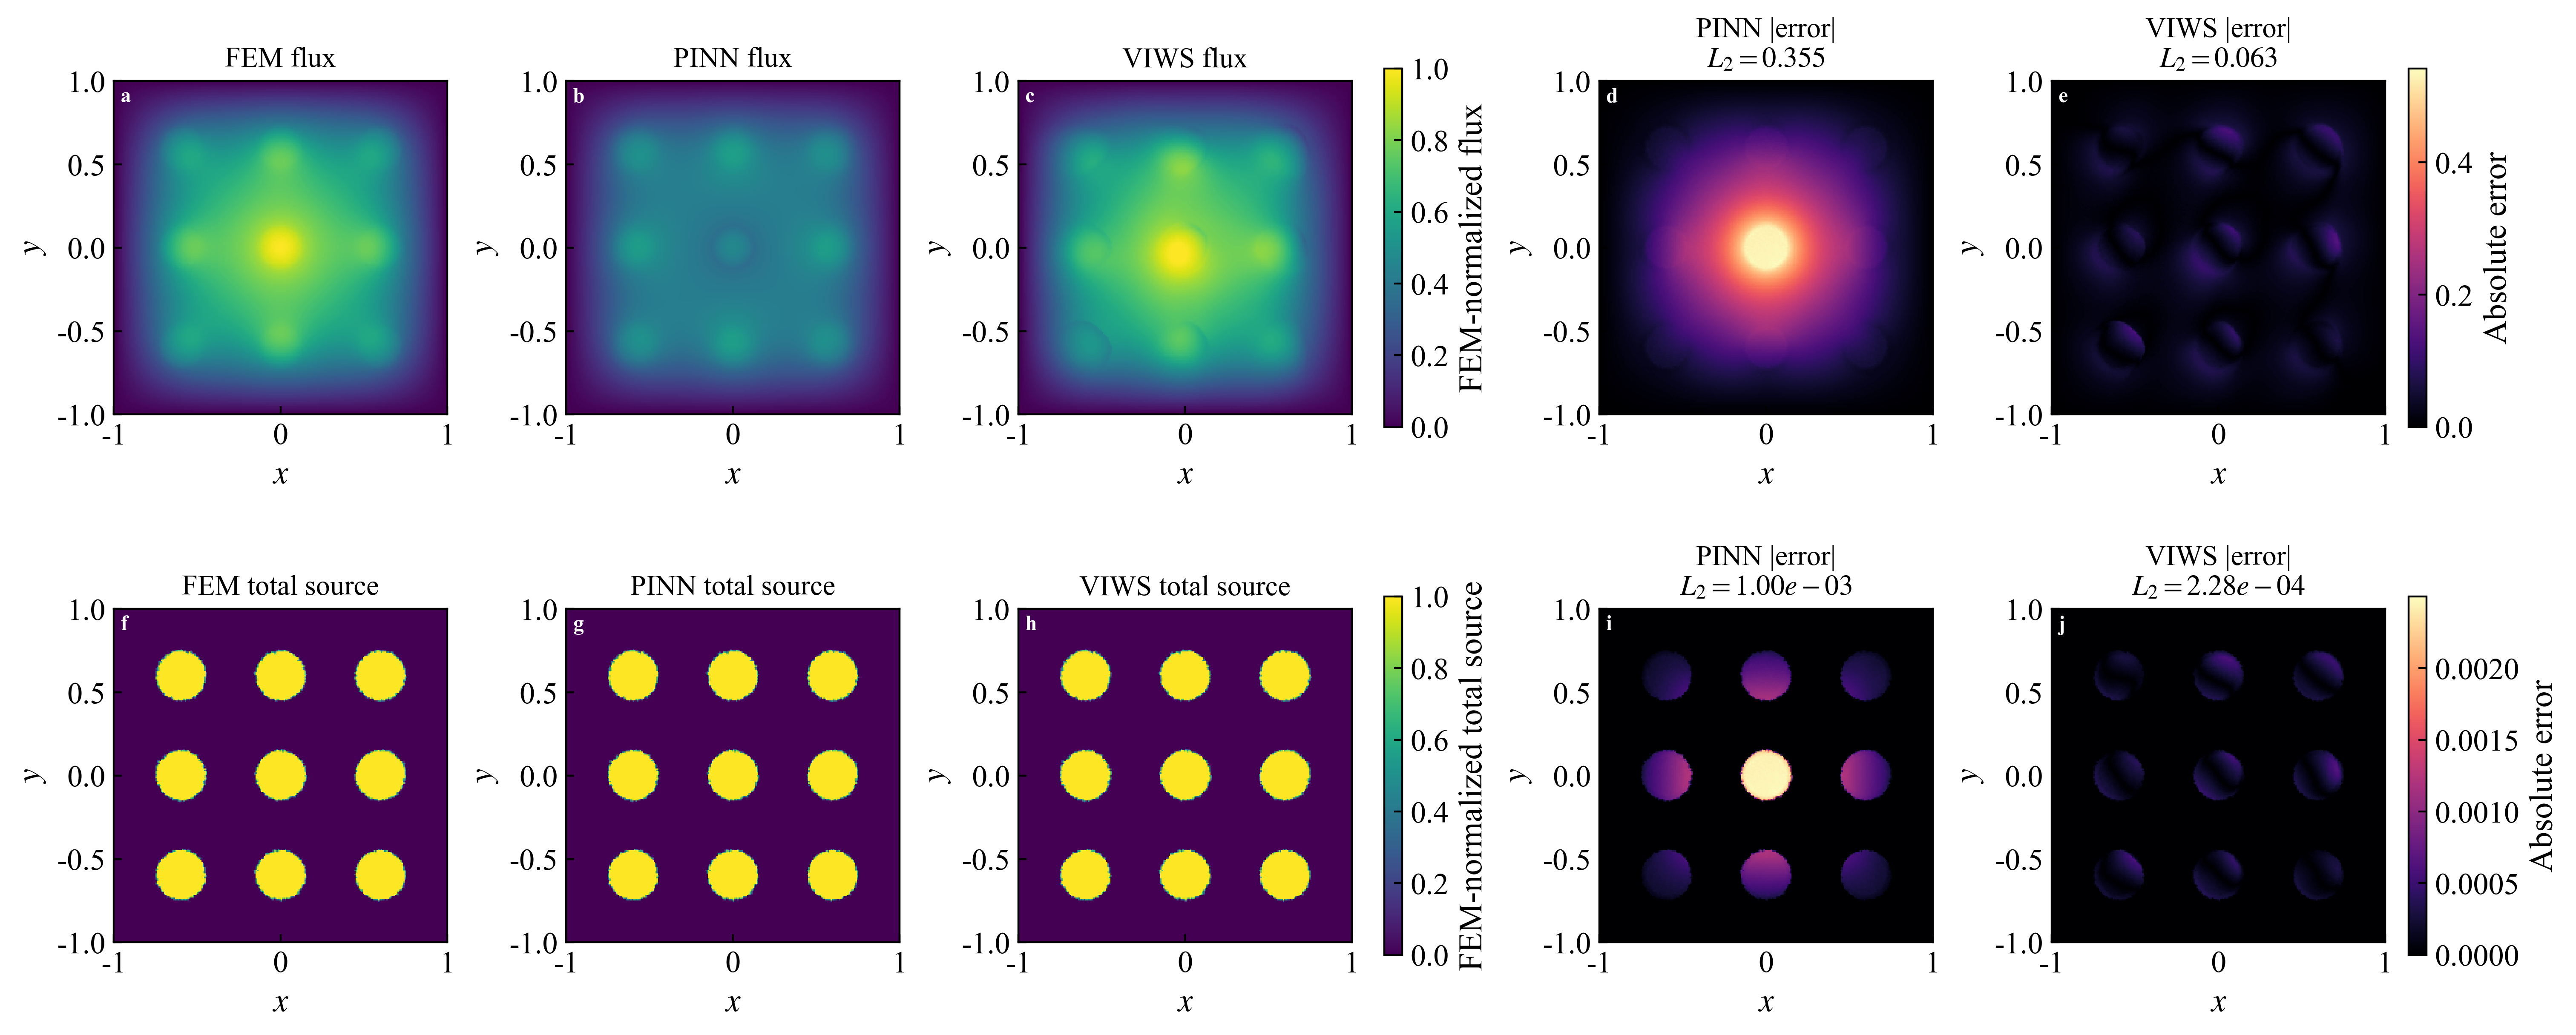
\includegraphics[width=\textwidth]{fig/figure_14.png}
\caption{修订稿新增的轴向平均对比图。（a）--（e）为归一化通量场及绝对误差；（f）--（j）为归一化总源场及绝对误差。}
\label{fig:response_axial_average_zh}
\end{figure}
相应修改见第 \draftplaceholder{页码} 页（第 \draftplaceholder{行号} 行）。
\revisionlocation{第 4.3 节，新增轴向平均定义公式和轴向平均对比图。}

\subsection*{R2.S5 -- 具体意见 5：第 4.4 节}
\begin{reviewercomment}
该方法在问题规模和边界条件方面有哪些限制？网格能否扩展到整个燃料组件的尺度？
\end{reviewercomment}
\authorresponse 感谢审稿专家的这些意见。修订稿区分了数学可扩展性和数值验证范围。当前算例验证了 Dirichlet、Neumann 和混合边界；Robin 与周期边界尚未验证。方法不依赖有限元式单元连接，但仍需要域内、边界和确定点采样。组件均匀化尺度可由全域坐标网络表示，但本文没有验证 pin-resolved 三维组件或全堆模型，因此不将当前结果外推到这些尺度。相应修改见第 \draftplaceholder{页码} 页（第 \draftplaceholder{行号} 行）。
\revisionlocation{第 4.3--4.5 节相关范围说明；结论局限性段落。}

\subsection*{R2.S6 -- 具体意见 6：第 4.5 节}
\begin{reviewercomment}
“每个组件的宽度为 20, cm，外围反射层 290 的厚度也是 20, cm。”

\begin{enumerate}[label=\alph*.,leftmargin=2em]
\item “cm”前面的逗号似乎没有必要。
\item VIMS 模型输出的是逐点通量形状，还是每个组件对应一个能够生成各点通量形状的二维函数？请更详细地说明通量输出过程，以及生成不同分辨率通量所需的内存。
\item 燃料组件是否被划分为子区域？此外，燃料组件区域是否在材料参数上进行了均匀化？
\end{enumerate}
\end{reviewercomment}
\authorresponse 感谢审稿专家的这些意见。（a）单位已改为 $20\,\mathrm{cm}$。（b）这里的方法为 VIWS。每个能群使用一个覆盖完整四分之一堆芯的坐标到通量函数，并非每个组件保存独立函数。模型参数内存不随查询分辨率改变，但查询坐标、激活和输出数组随 $N_q$ 增长，输出规模为 $O(GN_q)$。我们使用双精度和全网格推理完成了 $100^2$、$200^2$、$400^2$、$800^2$ 测试；中位推理时间分别为 0.00996、0.03708、0.10664 和 0.42140 s，峰值显存分别为 58.379、207.426、793.580 和 3,151.043 MiB。（c）该基准采用组件均匀化两群常数，$\Omega_1$--$\Omega_4$ 表示组件/反射层材料类别，不解析棒、气隙、包壳和慢化剂子区。

下面给出实测的分辨率--资源关系。全部数据来自三次纯推理重复；模型内存保持不变，而坐标、激活和输出所需内存随查询网格增大。

\begin{table}[H]
\centering
\small
\caption{两群 2D-IAEA 算例的分辨率相关全网格推理成本。}
\label{tab:response_iaea_memory_zh}
\renewcommand{\arraystretch}{1.15}
\begin{tabularx}{\textwidth}{@{}lrrrr@{}}
\toprule
查询网格 & 查询点数 & 推理时间 & 峰值 GPU 显存 & 输出/模型内存 \\
\midrule
$100^2$ & 10,000 & 0.00996 [0.00992, 0.00998] s & 58.379 MiB & 0.153 / 0.251 MiB \\
$200^2$ & 40,000 & 0.03708 [0.03705, 0.03727] s & 207.426 MiB & 0.610 / 0.251 MiB \\
$400^2$ & 160,000 & 0.10664 [0.10624, 0.11698] s & 793.580 MiB & 2.441 / 0.251 MiB \\
$800^2$ & 640,000 & 0.42140 [0.42136, 0.42252] s & 3,151.043 MiB & 9.766 / 0.251 MiB \\
\bottomrule
\end{tabularx}
\end{table}
相应修改见第 \draftplaceholder{页码} 页（第 \draftplaceholder{行号} 行）。
\revisionlocation{第 4.5 节几何、输出与内存说明；新增分辨率推理内存表。}

\subsection*{R2.S7 -- 具体意见 7：第 4.5 节}
\begin{reviewercomment}
“有效增殖因子 $k_{\mathrm{eff}}$ 被视为待优化的全局参数，并与神经网络权重一起更新 [45]。”

建议说明如何在同一个 VIWS 模型中同时得到通量和增殖因子的具体细节。
\end{reviewercomment}
\authorresponse 感谢审稿专家的这些意见。修订稿现已说明联合求解过程。快群和热群分别由两个全域通量网络表示，$k_{\mathrm{eff}}$ 作为独立标量从 1.0 初始化，并通过 $1/k_{\mathrm{eff}}$ 同时进入两群裂变源项。该结构化网格算例取 $v=1$，变上限积分残差直接采用累积数值积分，因此此算例不训练原函数辅助网络。两个通量网络与 $k_{\mathrm{eff}}$ 由同一 Adam--L-BFGS 流程联合更新。快群平均通量与目标值 1 之间的平方归一化约束用于固定特征函数尺度并排除零解。FEM 的 $k_{\mathrm{eff}}$ 仅用于训练后的误差评价，不作为监督信息。相应修改见第 \draftplaceholder{页码} 页（第 \draftplaceholder{行号} 行）。
\revisionlocation{第 3.4 节归一化损失与训练伪代码；第 4.5 节归一化公式及联合优化说明。}

\enlargethispage{3\baselineskip}
\vspace{0.5em}
% AUTOFILL:ZH_CLOSING:BEGIN
再次感谢编辑和审稿专家的建设性意见。当前回复包仍含明确标出的训练成本占位符；在相关独立重复实验完成并核验后，我们将更新表格、摘要和对应回复，再提交最终版本。
% AUTOFILL:ZH_CLOSING:END

\begin{flushright}
谨致谢意\\
全体作者
\end{flushright}

\end{document}
